% **************************************************
% Document Class Definition
% **************************************************
\documentclass[%
paper=A4,					% paper size --> A4 is default in Germany
twoside=true,				% onesite or twoside printing
openright,					% doublepage cleaning ends up right side
parskip=full,				% spacing value / method for paragraphs
chapterprefix=true,			% prefix for chapter marks
11pt,						% font size
headings=normal,			% size of headings
bibliography=totoc,			% include bib in toc
listof=totoc,				% include listof entries in toc
titlepage=on,				% own page for each title page
captions=tableabove,		% display table captions above the float env
draft=false,				% value for draft version
]{scrreprt}%


% **************************************************
% Debug LaTeX Information
% **************************************************
%\listfiles


% **************************************************
% Commands and packages
% **************************************************
% **************************************************
% Information and Commands for Reuse
% **************************************************
\newcommand{\thesisTitle}{Genome Analysis Methods using Long Read Nanopore Sequencing}
\newcommand{\thesisName}{Pay Giesselmann}
\newcommand{\thesisDegree}{M.Eng.}
\newcommand{\thesisSubject}{Dissertation}
\newcommand{\thesisDate}{October 23, 2019}
\newcommand{\thesisVersion}{My First Draft}

\newcommand{\thesisFirstReviewer}{Knut Reinert}
\newcommand{\thesisFirstReviewerUniversity}{\protect{Free University of Berlin}}
\newcommand{\thesisFirstReviewerDepartment}{Department of Reviewer}
\newcommand{\thesisFirstReviewerCity}{Berlin}

\newcommand{\thesisSecondReviewer}{John Doe}
\newcommand{\thesisSecondReviewerUniversity}{\protect{Reviewer University}}
\newcommand{\thesisSecondReviewerDepartment}{Department of Reviewer}
\newcommand{\thesisSecondReviewerCity}{City of Reviewer}

\newcommand{\thesisFirstSupervisor}{Knut Reinert}
\newcommand{\thesisSecondSupervisor}{Alexander Meissner}
\newcommand{\thesisThirdSupervisor}{Franz-Josef M\"uller}

\newcommand{\thesisUniversity}{\protect{Free University of Berlin}}
\newcommand{\thesisUniversityDepartment}{Department of Mathematics and Computer Science}
\newcommand{\thesisUniversityInstitute}{Institut for Computer Science}
\newcommand{\thesisUniversityGroup}{Reinert Lab}
\newcommand{\thesisUniversityCity}{Berlin}
\newcommand{\thesisUniversityStreetAddress}{Takustra\ss{}e 9}
\newcommand{\thesisUniversityPostalCode}{14195}

\newcommand{\thesisOrganization}{\protect{Max-Planck-Institue for Molecular Genetics}}
\newcommand{\thesisOrganizationDepartment}{Department of Genome Regulation}
\newcommand{\thesisOrganizationGroup}{Meissner Lab}
\newcommand{\thesisOrganizationCity}{Berlin}
\newcommand{\thesisOrganizationStreetAddress}{Ihnestra\ss{}e 63-73}
\newcommand{\thesisOrganizationPostalCode}{14195}

\newcommand{\biorxiv}{bioRxiv}
\newcommand{\Biorxiv}{BioRxiv}
% **************************************************
% Load and Configure Packages
% **************************************************
\usepackage[utf8]{inputenc}		% defines file's character encoding
\usepackage[english]{babel} % babel system, adjust the language of the content
\usepackage[					% clean thesis style
figuresep=colon,%
sansserif=false,%
hangfigurecaption=false,%
hangsection=true,%
hangsubsection=true,%
colorize=full,%
colortheme=bluemagenta,%
bibsys=bibtex,%
bibfile=zotero_refs,%
%bibstyle=alphabetic,%
bibstyle=numeric,
]{cleanthesis}

\hypersetup{					% setup the hyperref-package options
	pdftitle={\thesisTitle},	% 	- title (PDF meta)
	pdfsubject={\thesisSubject},% 	- subject (PDF meta)
	pdfauthor={\thesisName},	% 	- author (PDF meta)
	plainpages=false,			% 	-
	colorlinks=false,			% 	- colorize links?
	pdfborder={0 0 0},			% 	-
	breaklinks=true,			% 	- allow line break inside links
	bookmarksnumbered=true,		%
	bookmarksopen=true			%
}

%% Listings
\usepackage{listings}
\usepackage{xcolor}

\definecolor{codegreen}{rgb}{0,0.6,0}
\definecolor{codegray}{rgb}{0.5,0.5,0.5}
\definecolor{codepurple}{rgb}{0.58,0,0.82}
\definecolor{backcolour}{rgb}{0.95,0.95,0.92}

\lstdefinestyle{mystyle}{
	backgroundcolor=\color{backcolour},   
	commentstyle=\color{codegreen},
	keywordstyle=\color{magenta},
	numberstyle=\tiny\color{codegray},
	stringstyle=\color{codepurple},
	basicstyle=\ttfamily\footnotesize,
	breakatwhitespace=false,         
	breaklines=true,                 
	captionpos=b,                    
	keepspaces=true,                 
	numbers=left,                    
	numbersep=5pt,                  
	showspaces=false,                
	showstringspaces=false,
	showtabs=false,                  
	tabsize=2
}

\lstset{style=mystyle}



% **************************************************
% Document CONTENT
% **************************************************
\begin{document}
	% --------------------------
	% rename document parts
	% --------------------------
	\renewcaptionname{english}{\figurename}{Fig.}
	\renewcaptionname{english}{\tablename}{Tab.}
	
	% --------------------------
	% Front matter
	% --------------------------
	\pagenumbering{roman}					% roman page numbing (invisible for empty page style)
	\pagestyle{empty}						% no header or footers
	% ------------------------------------  --> main title page
\begin{titlepage}
	\pdfbookmark[0]{Titlepage}{Titlepage}
	\tgherosfont
	\centering

	{\Large \thesisUniversity} \\[4mm]
	%\includegraphics[width=6cm]{figures/pdf/logo} \\[2mm]
	\textsf{\thesisUniversityDepartment} \\
	\textsf{\thesisUniversityInstitute} \\
	%\textsf{\thesisUniversityGroup} \\

	\vfill
	{\large \thesisSubject} \\[5mm]
	{\LARGE \color{ctcolortitle}\textbf{\thesisTitle} \\[10mm]}
	{\large submitted by} \\[5mm]
	{\Large \thesisName} \\

	\vfill
	\begin{minipage}[t]{.27\textwidth}
		\raggedleft
		\textit{1. Reviewer}
	\end{minipage}
	\hspace*{15pt}
	\begin{minipage}[t]{.65\textwidth}
		{\Large \thesisFirstReviewer} \\
	  	{\small \thesisFirstReviewerUniversity} \\[-1mm]
		{\small \thesisFirstReviewerCity}
	\end{minipage} \\[5mm]
	\begin{minipage}[t]{.27\textwidth}
		\raggedleft
		\textit{2. Reviewer}
	\end{minipage}
	\hspace*{15pt}
	\begin{minipage}[t]{.65\textwidth}
		{\Large \thesisSecondReviewer} \\
	  	{\small \thesisSecondReviewerUniversity} \\[-1mm]
		{\small \thesisSecondReviewerCity}
	\end{minipage} \\[10mm]
	\begin{minipage}[t]{.27\textwidth}
		\raggedleft
		\textit{Supervisors}
	\end{minipage}
	\hspace*{15pt}
	\begin{minipage}[t]{.65\textwidth}
		\thesisFirstSupervisor\ \\ \thesisSecondSupervisor\ \\ \thesisThirdSupervisor
	\end{minipage} \\[10mm]

	\thesisDate \\

\end{titlepage}


\newpage\null\thispagestyle{empty}\newpage


% ------------------------------------  --> lower title
\hfill
\vfill
{
	\small
	\textbf{\thesisDegree\ \thesisName} \\
	\textit{\thesisTitle} \\
	\thesisSubject, \thesisDate \\
	Reviewers: \thesisFirstReviewer\ and \thesisSecondReviewer \\
	Supervisors: \thesisFirstSupervisor\ and \thesisSecondSupervisor\ and \thesisThirdSupervisor \\[1.0em]
	% --- Max-Planck-Institute
	\textbf{\thesisOrganization} \\
	\thesisOrganizationDepartment \\
	\textit{\thesisOrganizationGroup} \\
	\thesisOrganizationStreetAddress \\
	\thesisOrganizationPostalCode\ \thesisOrganizationCity \\[1.0em]
	% --- Free University of Berlin
	\textbf{\thesisUniversity} \\
	\thesisUniversityDepartment \\
	\thesisUniversityInstitute \\
	\textit{\thesisUniversityGroup} \\
	\thesisUniversityStreetAddress \\
	\thesisUniversityPostalCode\ \thesisUniversityCity
}
			% INCLUDE: all titlepages
	\cleardoublepage
	
	\pagestyle{plain}						% display just page numbers
	\pdfbookmark[0]{Abstract}{Abstract}
\chapter*{Abstract}
\label{sec:abstract}
\vspace*{-10mm}

\blindtext

\vspace*{20mm}

{\usekomafont{chapter}Zusammenfassung}\label{sec:abstract-diff} \\

\blindtext
			% INCLUDE: the abstracts (english and german)
	\cleardoublepage
	\pdfbookmark[0]{Bibliographic Information}{Bibliographic Information}
\chapter*{Bibliographic Information}
\label{sec:bib}
\vspace*{-10mm}


This thesis is based on the following publications:

\textbf{Pay Giesselmann}, Sara Hetzel, Franz-Josef Müller, Alexander Meissner and Helene Kretzmer. \textit{Nanopype: a modular and scalable nanopore data processing pipeline}. \textbf{Bioinformatics}, 2019.


\textbf{Pay Giesselmann}*, Björn Brändl*, Etienne Raimondeau, Rebecca Bowen, Christian Rohrandt, Rashmi Tandon, Helene Kretzmer, Günter Assum, Christina Galonska, Reiner Siebert, Ole Ammerpohl, Andrew Heron, Susanne A. Schneider, Julia Ladewig, Philipp Koch, Bernhard M. Schuldt, James E. Graham, Alexander Meissner and Franz-Josef Müller. \textit{Analysis of short tandem repeat expansions and their methylation state with nanopore sequencing}. \textbf{Nature Biotechnology}, 2019. *joint first authorship







	\cleardoublepage
	\pdfbookmark[0]{Acknowledgement}{Acknowledgement}
\chapter*{Acknowledgement}
\label{sec:acknowledgement}
\vspace*{-10mm}

\begin{figure}[h]
	\centering
	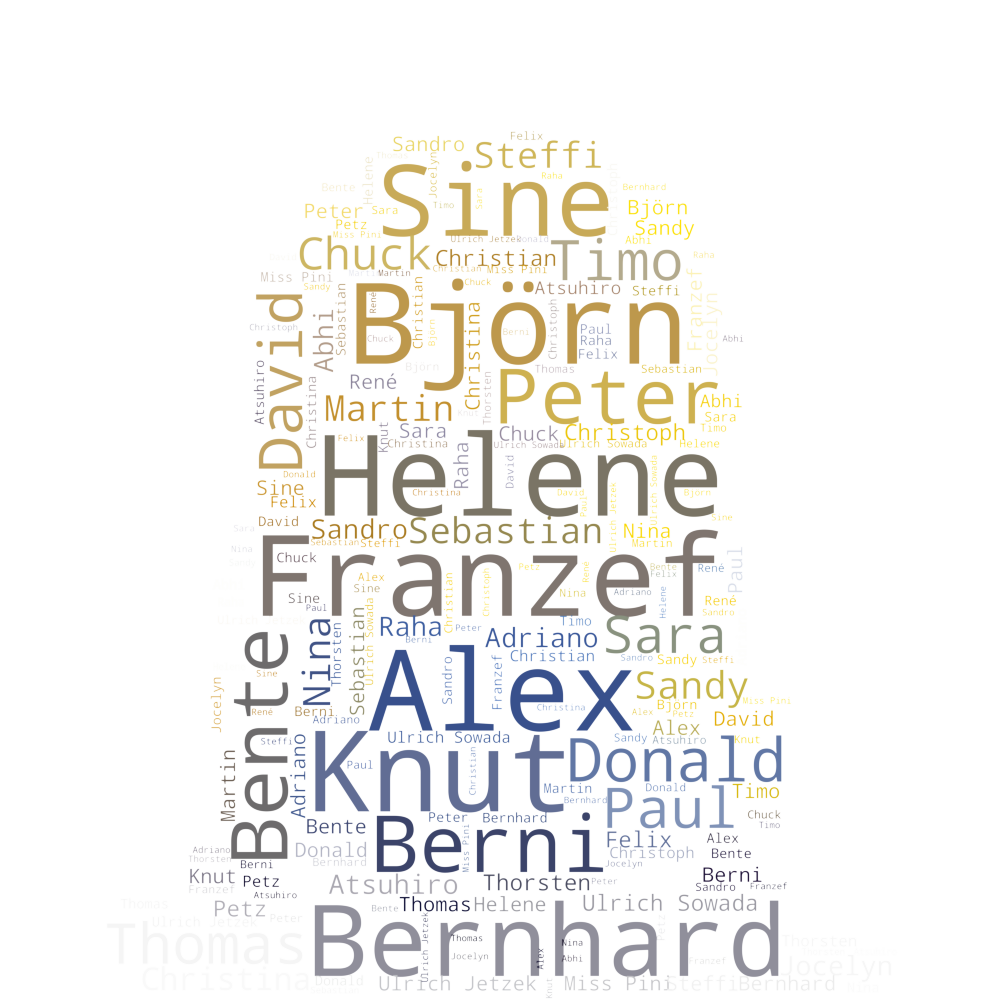
\includegraphics[width=0.75\textwidth]{util/ack.png}
\end{figure}

 	% INCLUDE: acknowledgement
	\cleardoublepage
	

	
	%
	\setcounter{tocdepth}{2}				% define depth of toc
	\tableofcontents						% display table of contents
	\cleardoublepage
	
	% --------------------------
	% Body matter
	% --------------------------
	\pagenumbering{arabic}					% arabic page numbering
	\setcounter{page}{1}					% set page counter
	\pagestyle{maincontentstyle} 			% fancy header and footer
	
	\chapter{Introduction}
\label{sec:intro}

%\cleanchapterquote{You can’t do better design with a computer, but you can speed up your work enormously.}{Wim Crouwel}{(Graphic designer and typographer)}


\section{Motivation}
\label{sec:intro:motivation}

\section{Results}
\label{sec:intro:results}


\section{Structure}
\label{sec:intro:structure}


\textbf{Chapter \ref{sec:nanopype}} \\[0.2em]
\blindtext


	\chapter{State of the Art}
\label{sec:state_of_art}
	\chapter{Nanopype Processing Pipeline}
\label{sec:nanopype}

Long-read third-generation nanopore sequencing enables researchers to now address a range of questions that are difficult to tackle with short read approaches. The rapidly expanding user base and continuously increasing throughput have sparked the development of a growing number of specialized analysis tools. However, streamlined processing of nanopore datasets using reproducible and transparent workflows is still lacking. Here we present Nanopype, a nanopore data processing pipeline that integrates a diverse set of established bioinformatics software while maintaining consistent and standardized output formats. Seamless integration into compute cluster environments makes the framework suitable for high-throughput applications. As a result, Nanopype facilitates comparability of nanopore data analysis workflows and thereby should enhance the reproducibility of biological insights. Nanopype is available at \textit{https://github.com/giesselmann/nanopype}.

\begin{figure}[h]
    \centering
    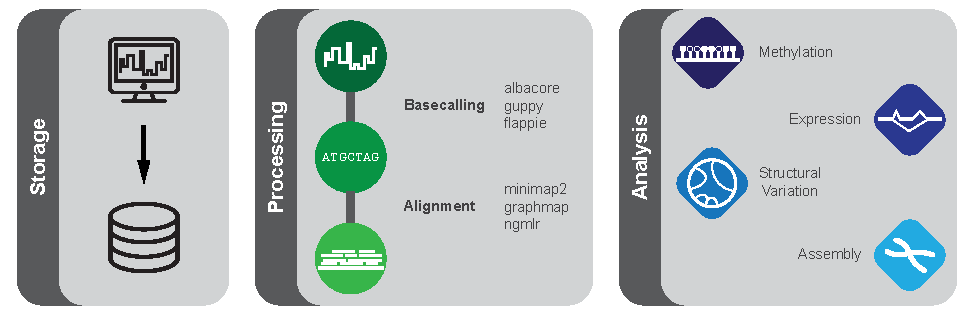
\includegraphics[width=1.0\textwidth]{figures/nanopype/GA.pdf}
    \label{fig:nanopype:ga}
\end{figure}

\textbf{Note:} This chapter is based on the publication P. Giesselmann et al. \textit{Nanopype: a modular and scalable nanopore data processing pipeline}, Bioinformatics, 2019 and contains text from the original paper.

The chapter starts with a brief \textbf{background} in \ref{sec:nanopype:background} followed by high-level pipeline \textbf{design} decisions covering storage, tool encapsulation and reproducibility in section \ref{sec:nanopype:design}.
The \textbf{installation} section \ref{sec:nanopype:installation} illustrates the setup and configuration of the pipeline in different environments. Grouped into \textbf{modules} individual tools are highlighted in section \ref{sec:nanopype:modules}.
Finally the \textbf{usage} on a daily production level is outlined in section \ref{sec:nanopype:usage}.


\section{Background}
\label{sec:nanopype:background}
Third-generation sequencing techniques are currently introducing new perspectives to the field of genome analysis by generating previously unattainable read lengths with averages in the tens of thousands of nucleotides. Among other devices distributed by Oxford Nanopore Technologies (ONT), the MinION in particular is gaining prominence. In brief, the nanopore sequencing process is based on guiding a nucleotide polymer through a pore inserted in a membrane while measuring a change in ionic current as a proxy signal over time. This signal is then interpreted to determine the underlying DNA or RNA sequence. The nanopore technology enables direct readout of sequences from individual DNA or RNA molecules including base modifications since no synthesis or amplification is required.

Due to constant development and improvement of applications, frequent reprocessing of the raw signal and downstream data is necessary. Thus, novel archiving and processing strategies are needed for data storage and handling that scale with the large amount of data produced by the MinION sequencer. This will be even more relevant as higher throughput devices such as the PromethION become more widely available. Furthermore, a limiting factor of the applicability of this new technology are the currently available, research-grade software packages for nanopore long-read data analyses. These tend to be difficult to install and require complex software environments. Despite the growing number of recently developed algorithms \cite{Magi2018}, primary data processing remains challenging due to stand alone tools without congruent data formats and requirements. 
Current examples of nanopore data processing pipelines are Katuali\footnote{github.com/nanoporetech/katuali} for basecalling and assembly and Pinfish\footnote{github.com/nanoporetech/pipeline-pinfish-analysis} for RNA isoform detection from cDNA and direct RNA sequencing experiments. However they have been developed to perform specific analysis workflows without integrated handling of the critical raw data storage or version control of wrapped tools.

To overcome these issues, we have developed Nanopype, a pipeline designed explicitly for streamlined and automated nanopore long read processing. Apart from the integration of essential base calling, quality control, and alignment tools, we facilitate a set of published analysis applications for barcode demultiplexing, DNA methylation readout, structural variant calling, RNA isoform detection and genome assembly. 
Based on the Snakemake engine \cite{Koester2012} our method integrates established error handling and uniform output structures across multiple experiments. Furthermore, Nanopype can be run in a parallel setup on both, single computers and server clusters. Deployed as a python module, Nanopype is mostly build from source with encapsulated routines to simplify the initial setup and integration into existing environments. Additionally, we provide Singularity images for all modules and an automatically built all-in-one Docker container. This enables the usage of the pipeline for both, less bioinformatically experienced experimental scientists and bioinformaticians. Lastly, Nanopype provides a well-defined framework for standardized processing independent of the underlying operating system.




\section{Design}
\label{sec:nanopype:design}
Nanopype’s core element is a modular setup to easily update existing tools and to seamlessly integrate the latest developments. Nonetheless, each pipeline release is freezing the included tool versions to guarantee reproducible results. In a nutshell, Nanopype has been designed around three key components: raw data storage, tool encapsulation and standardized directory structures that mirror the applied toolchain.

\subsection{Storage}
\label{subsec:nanopype:storage}
The first core design component is the consistent storage of the raw signal data from any ONT sequencer. 
Raw nanopore reads are stored in FAST5 files, an ONT specification of the universal HDF5 file format. Initially the sequencers exported one file per read, resulting in hundreds of thousands of files per sequencing run. 
The number of files generated could, especially on Linux file systems, disrupt background services such as nightly mirrors and backups.
Nanopype is backward compatible with datasets of single read FAST5 files, for which we provide a module to import and package single reads into TAR archive batches.

More recently ONT utilized the full functionality of the HDF5 format with groups (comparable to directories), datasets (structured arrays of primitive data types) and attributes (single values for meta information) and released the multi-read-FAST5 format. The new format typically groups 4000 reads into a single file, resulting in notable improvements regarding copy and synchronization tasks.


\begin{itemize}
	\item syncthing
	\item separation of raw and processed data
	\item user management
	\item archive
\end{itemize}



\begin{figure}[h]
	\centering
	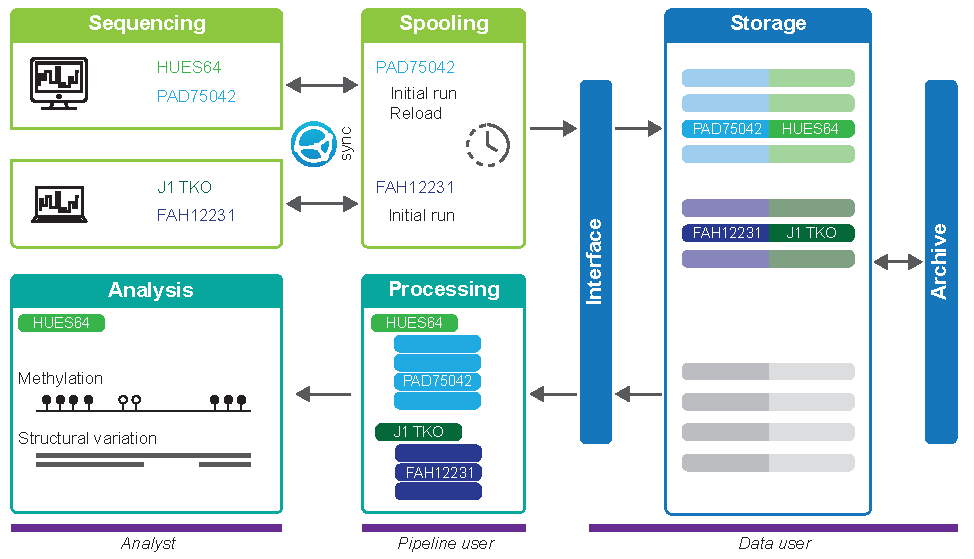
\includegraphics[width=1.0\textwidth]{figures/nanopype/storage.pdf}
	\captionsetup{format=plain}
	\caption[Nanopype data flow]{}
	\label{fig:nanopype:storage}
\end{figure}

This raw data archive forms the basis for any downstream analyses and enables smooth re-processing of legacy datasets as soon as improved basecalling algorithms become available.

\subsection{Encapsulation}
\label{subsec:nanopype:encapsulation}
The installation of experimental software packages still being actively developed with complex library dependencies can be time-consuming but remains essential to make use of the current-generation nanopore analysis workflows. On a base level, Nanopype uses Snakemake rules to wrap the build from source and installation process of its dependencies and therefore does not require root privileges for the setup on common Linux and MacOS systems. The build from source is the most customizable setup option and moreover allows the integration into complex, preexisting environments.
Internal wrappers are used to automatically build and deploy Singularity images for preset modules and pipeline versions. This mechanism enables the complete function set of Snakemake and Nanopype while only requiring a system-wide Python and Singularity installation.
An all-in-one Docker container is provided, wrapping the entire pipeline into a single environment. Primarily aimed for stand-alone usage, Windows systems, and for initial testing, this method does not offer support for cluster computation. Consistent versioning ensures reproducibility independent of the installation method.

\begin{itemize}
	\item discuss container size on distributed systems
	\item more details on Docker vs. Singularity
\end{itemize}


\subsection{Transparency}
\label{subsec:nanopype:transparency}
Nanopype follows the Snakemake concept of output file driven computation: a single user command typically provokes transparent processing of any required intermediate result. Preexisting tools are integrated into consistent workflows and provide standard output formats to connect to workflows of established next-generation sequencing data analysis tools. The processing and subsequent output is intuitively organized in modules and underlying application directories.




\section{Installation}
\label{sec:nanopype:installation}

\subsection{Source}

\begin{itemize}
	\item dependencies
	\item build rules
	\item tests
\end{itemize}

\subsection{Container}


\lstinputlisting[language=docker, caption=Staged Docker build, label=lst:nanopype:docker]{listings/nanopype/docker_staged.txt}


\begin{itemize}
	\item Docker
	\item Singularity
	\item Staged builds \ref{lst:nanopype:docker}
\end{itemize}

\subsection{Configuration}

\begin{itemize}
	\item environment
	\item workflow
	\item profiles
	\item cluster
	\subitem shadow prefix
	\item GPU support
\end{itemize}




\section{Modules}
\label{sec:nanopype:modules}
Nanopype’s backbone consists of a set of modules that resolve a specific task, like basecalling, alignment or further downstream analyses. If available, alternative applications are provided for the same task and grouped into a module with a coherent output format. Integrating first and foremost low-level nanopore data processing applications provided by ONT, established community developed software packages have been included in the first Nanopype release, as well.

\subsection{Basecalling}
\label{subsec:nanopype:basecalling}
The basecalling module translates raw nanopore signals into nucleotide sequences and is utilized by most subsequent pipeline layers. With the initial release, we include the established packages Guppy, Albacore, and Flappie, all provided by ONT \cite{Wick2019}. The default basecaller package is set to the recently released Guppy. Albacore is supported for backward compatibility but deprecated by ONT. The experimental Flappie is ONT’s first DNA methylation-aware basecaller. It extends the usual four-letter nucleotide alphabet by a fifth letter for methylated cytosine in CpG contexts. For all basecallers, the output is either the standardized FASTA or FASTQ and supplemented by us with a basic quality control summary.

\subsection{Alignment}
\label{subsec:nanopype:alignment}
The core functionality of the pipeline is the alignment of reads against a reference genome or draft assembly. Here, we provide three different aligners with distinct advantages, which make them favorable for different applications downstream. While Minimap2 \cite{Li2018} is a fast, low memory footprint solution suitable for both DNA and RNA alignments, GraphMap \cite{Sovic2016} is a sensitive aligner but with comparably high memory requirements. NGMLR \cite{Sedlazeck2018} is the recommended tool for the structural variation module. Any combination of basecalling, alignment, and reference genome is supported and reports BAM format files.

\begin{itemize}
	\item sorting
	\item merging of many files
\end{itemize}

\subsection{DNA methylation}
\label{subsec:nanopype:methylation}
Sequencing without prior DNA amplification enables the direct readout of DNA base modifications. The current state of the art approach, Nanopolish \cite{Simpson2017} as well as the more experimental flip-flop basecaller Flappie, are incorporated into Nanopype. Subsequently, Nanopype splits Flappie’s atypical sequence output into standard FASTQ and methylation status. DNA methylation at CpG dinucleotides of both tools is reported in a table format for single reads. Furthermore, we provide common bedGraph and bigWig files for genome-wide methylation tracks and thus enable downstream processing using established workflows, e.g., calling of differential methylated regions and comparison to bisulfite sequencing.

\begin{itemize}
	\item tracks
	\item single read tracks
\end{itemize}

\subsection{Structural variation}
\label{subsec:nanopype:sv}
Detection and characterization of structural variation play a central role in cancer research and population genetics. Long read sequencing particularly facilitates investigation of variants with unprecedented accuracy and resolution. Therefore, Nanopype encompasses the variant caller Sniffles \cite{Sedlazeck2018} and provides output in the standard variant calling format (VCF).

\subsection{Transcriptome}
\label{subsec:nanopype:transcriptom}
Another application of the long-read nanopore technology is sequencing of cDNA and RNA molecules directly. Recovery of full-length transcripts enables, for instance, the detection of alternatively spliced isoforms and is implemented in Nanopype using the Pinfish package. The output of polished transcripts is provided in the GFF format.


Miscellaneous: Complemented by samtools \cite{Li2009}, bedtools \cite{Quinlan2010} and UCSCtools \cite{Kent2010} our pipeline establishes a comprehensive framework for ONT sequencing data processing.




\section{Usage}
\label{sec:nanopype:usage}
Due to the functional range of Nanopype, dependent on the operating system, and selected installation method the setup can require advanced information technology knowledge. However, after deployment, the subsequent usage is straightforward given basic command line understanding. Complete Nanopype workflows can be executed with a single concise command line call. For instance, local processing of multiple flow cells into a collective genome-wide methylation track of at least 5x coverage on reference hg38 requires only the following line:

\begin{lstlisting}[language=sh, caption=Snakemake example]
snakemake --snakefile ~/nanopype/Snakefile methylation/nanopolish/ngmlr/guppy/sample.5x.hg38.bw
\end{lstlisting}

This command invokes basecalling, alignment and methylation detection using declared tools without further user interaction. The basecalling and alignment outputs are kept and can be reused to avoid redundant processing.

\begin{itemize}
	\item tag concept
	\item special tag introduction
\end{itemize}

\subsection{Batch processing}
The automatic distribution of workflows into independent batches enables efficient handling of high-throughput experiments. This feature becomes particularly relevant for scaling in cluster environments and most importantly in case of terminated or failed batches. As a result, only failed batches require reprocessing by resuming the workflow from where it left off, using the same command which enhances the overall error robustness.
The source and Singularity versions of Nanopype do not interfere with the extensive cluster support of Snakemake.

\begin{itemize}
	\item raw signal batches
	\item temporary data
	\item non batch modules e.g. sv
\end{itemize}

\subsection{Barcoding}

Demultiplexing: Barcoded sequencing allows pooling of multiple samples on a single flow-cell. The demultiplexing module uses Deepbinner \cite{Wick2018} to assign a barcode label to the individual reads. Thus, sequencing of comparable small bacterial genomes can be efficiently parallelized to use the available sequencing depth optimally.

Indexing the content of both, packaged and multi-FAST5 output enables the fast retrieval of individual reads. 

\subsection{Logging and Reports}

\begin{itemize}
	\item cluster job logging
	\item TODO: implement log of config values into tagged logfile
\end{itemize}




\section{Summary}
\label{sec:nanopype:summary}
Here we present Nanopype, a modular and easy-to-use data processing pipeline with a detailed online documentation, specifically designed to handle nanopore sequenced long-read data.
Nanopype provides end-to-end processing of the raw sequencer signal into standard data formats and consequently closes the gap to downstream next-generation sequencing algorithms. Single command invocations of entire workflows reduce the hands-on-time for users to receive the desired output. Implicitly, this also lowers the potential of user mistakes and deviations in processing of multiple data sets. As a consequence, workflows are easier to reproduce with fixed versions among datasets or repeated with improved tool releases on existing ones.
Nanopype is implemented as a python package and additionally provides pre-built and versioned Singluarity and Docker images, making it favorable for effective usage in cluster and single computer environments. The pipeline design ensures portability and version controlled usage of the implemented tools, to enable consistent results across platforms.



	\chapter{Nanopore Signal Analysis}
\label{sec:signal}

\begin{itemize}
	\item basics set with pipeline
	\item need to understand signal, contrast to 2nd gen.
	\item tombo, squiggle-kit?
	\item custom, easy to configure
	\item python for fast prototyping
\end{itemize}

\section{Normalization}
\label{sec:signal:normalization}

\begin{itemize}
	\item mean/std vs median/MAD (cite tombo)
	\item min-max normalization
	\item polyfit?
	\item smoothing with grayscale morphological operations
\end{itemize}

\section{Segmentation and Alignment}
\label{sec:signal:alignment}



\begin{itemize}
	\item estimated event alignment
	\item seqan vs. edlib
	\item event length
	\item profile HMM for precise mapping
\end{itemize}
	\chapter{STRique Repeat Detection}
\label{cha:strique}

Expansions of short tandem repeats are genetic variants that have been implicated in several neuropsychiatric and other disorders, but their assessment remains challenging with current polymerase-based methods. Here we combine a CRISPR-Cas-based enrichment strategy for nanopore sequencing with an algorithm for raw signal analysis. Our method, termed \textit{STRique} for short tandem repeat identification, quantification and evaluation, integrates conventional sequence mapping of nanopore reads with raw signal alignment for the localization of repeat boundaries and a hidden Markov model based repeat counting mechanism. We demonstrate the precise quantification of repeat numbers in conjunction with the determination of CpG methylation states in the repeat expansion and in adjacent regions at the single-molecule level without amplification. Our method enables the study of previously inaccessible genomic regions and their epigenetic marks. \textit{STRique} is available at \textit{https://github.com/giesselmann/STRique}.

\begin{figure}[h]
    \centering
    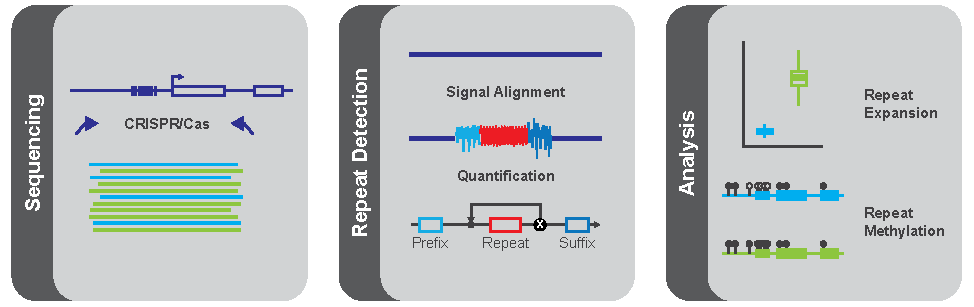
\includegraphics[width=1.0\textwidth]{figures/strique/GA.pdf}
    \label{fig:strique:ga}
\end{figure}

\textbf{Note:} This chapter is based on the publication P. Giesselmann et al. \textit{Analysis of short tandem repeat expansions and their methylation state with nanopore sequencing}, Nature Biotechnology, 2019 and contains text and figures from the original paper.

The chapter starts with a brief \textbf{background} in \ref{sec:strique:background}, followed by the evaluation of \textbf{sequenced based} repeat analysis in \ref{subsec:strique:seq_repeat_counts}. The development of an accurate \textbf{signal based} method is described in \ref{subsec:strique:sig_repeat_counts} and applied to patient samples with \textbf{c9orf72} and \textbf{FMR1} repeat expansions in \ref{subsec:strique:c9orf72}. Finally the DNA methylation detection on repeat and surrounding sequence is shown in \ref{sec:strique:modifications}.




\section{Background}
\label{sec:strique:background}

The expansion of unstable genomic Short Tandem Repeats (STRs) causes more than 30 Mendelian human disorders \cite{Gatchel2005}. An extended GGGGCC-repeat $ [(G_{4}C_{2})_{n}] $ within the C9orf72 gene is the most frequent monogenic cause of Frontotemporal Dementia and Amyotrophic Lateral Sclerosis c9FTD/ALS \cite{Paulson2018}. Similarly, accumulation of a CGG motif in the FMR1 gene underlies the Fragile X Syndrome, currently one of the most common identifiable genetic causes of mental retardation and autism \cite{Verkerk1991}. In both repeat expansion disorders, recent evidence has suggested pronounced inter- and intraindividual repeat variability as well as focal changes in DNA methylation to modulate the disease phenotype \cite{Blitterswijk2013, Xi2013, Russ2015}.

Put STRs into context of other repeat classes.

Difficulties in quantifying repeat lengths. 

Observation of repetitive signal in NA12878 on c9orf72 locus in cell line.

\begin{figure}[h]
	\centering
	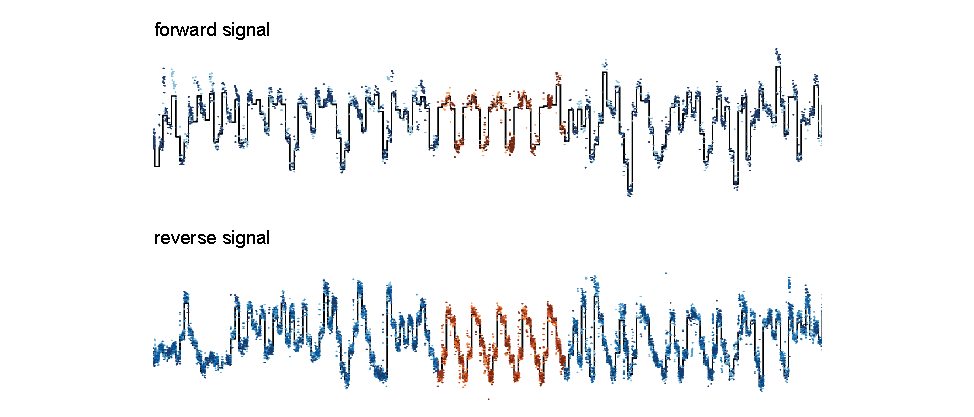
\includegraphics[width=1.0\textwidth]{figures/strique/signal.pdf}
	\captionsetup{format=plain}
	\caption[Nanopore raw signal of the C9orf72 STR in NA12878 cells]{Multi signal HMM alignment of publicly available raw traces from two forward and eight reverse strand reads from the NA12878 cell line shows matching signal pattern in all reads \cite{Jain2018}. Displayed are the current measurements as dots and the model signal as black line. Blue dots indicate current measurements identified as prefix or suffix sequence. Red dots indicate raw current measurements identified by \textit{STRique} as belonging to the C9orf72-$ (G_{4}C_{2})_{n} $-STR. \textit{STRique} detects in this case a $ (G_{4}C_{2})_{5} $-repeat.}
	\label{fig:strique:signal}
\end{figure}

To overcome current difficulties in characterizing expanded STRs we focused on three areas: i) optimization of nanopore sequencing and signal processing to capture STRs ii) development and implementation of a target enrichment strategy to increase efficiency and iii) integration of expansion measurements with CpG methylation at the single molecule level.
To enable a robust repeat analysis, we developed \textit{STRique}, a general-purpose signal processing algorithm for the exact quantification of STR numbers in raw nanopore signals.





\section{Repeat quantification}
\label{sec:strique:quantification}

Accurate counting of repeat lengths is a first step during investigation of short tandem repeats. While generally a sequence based approach appears desirable due to a lower implementation complexity, the following sections illustrate the need for a signal based algorithm to exactly quantify the length of a short tandem repeat based on nanopore sequencing.

\subsection{Sequence based repeat detection}
\label{subsec:strique:seq_repeat_counts}

To first benchmark existing repeat expansion counting methods we constructed, verified and nanopore sequenced plasmids with several synthetic $ [(G_{4}C_{2})_{n}] $-repeat lengths \cite{Mizielinska2014}. Current (May 2019) production grade (Guppy v3.0.3) software developed by Oxford Nanopore Technologies (ONT) was used to translate the nanopore raw signal into base-space representations. As a first baseline, we manually counted repeats for a subset of reads, exploiting the clear visibility of the repetitive signal pattern (Fig. \ref{fig:strique:signal}).



The analysis revealed, that current generation sequence based methods fail to satisfactorily resolve expanded STRs (Fig. \ref{fig:strique:count_seq_manual}).


\begin{figure}[h]
    \centering
    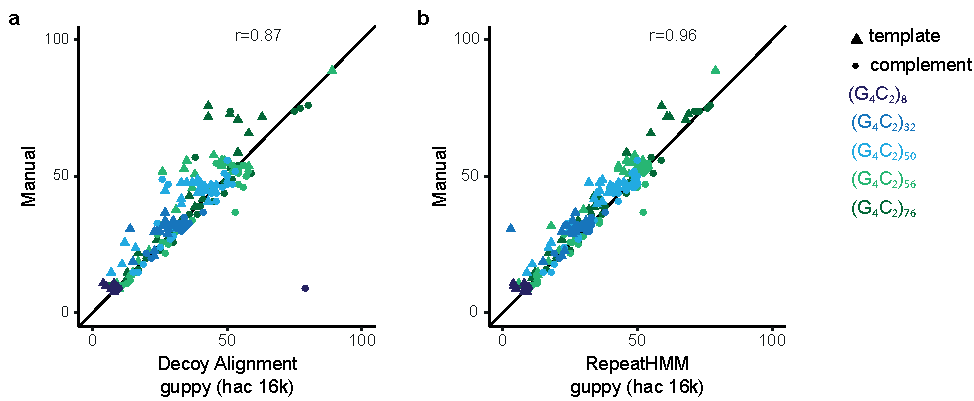
\includegraphics[width=1.0\textwidth]{figures/strique/count_seq_manual.pdf}
    \captionsetup{format=plain}
    \caption[Correlation and strand bias in STR analysis methods]{Manual counted set of plasmid reads on y-axis correlating with guppy basecalling and decoy alignment approach (\textbf{a}) and RepeatHMM (\textbf{b}) on x-axis. Only data points shown which could be evaluated with all three methods (n=15, 49, 45, 48, 47; Pearson correlation).}
    \label{fig:strique:count_seq_manual}
\end{figure}

\begin{figure}[h]
	\centering
	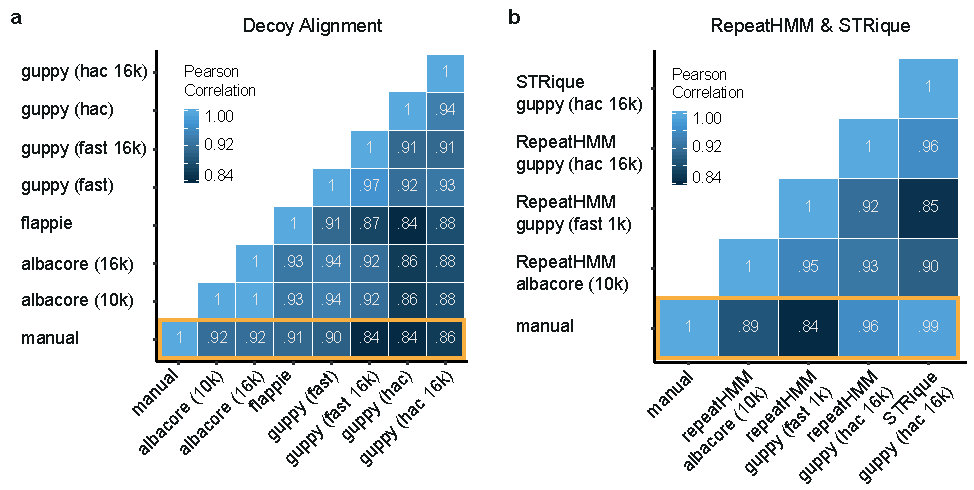
\includegraphics[width=1.0\textwidth]{figures/strique/count_sequence_corr.pdf}
	\captionsetup{format=plain}
	\caption[Correlation of sequence based STR detection methods]{\textbf{a}, Correlation of manual counted repeat lengths with sequence base methods. Decoy alignment against reference with 3-100 repeats with Albacore (window 10k and 16k), Guppy (fast and hac mode, 1k and 16k window size) and Flappie basecalling (n=204 reads). \textbf{b}, Correlation of manual count with RepeatHMM and \textit{STRique} results (n=204 reads).}
	\label{fig:strique:count_sequence_corr}
\end{figure}

The analysis’ results revealed that the current generation of general-purpose basecalling algorithms cannot satisfactorily resolve expanded STR sequences (Supplementary Fig. 4). For our purpose we systematically combined outputs from three ONT basecaller generations (Albacore, Flappie, Guppy) and different parameter sets with two current sequence based STR quantification approaches (Decoy Alignment18 and RepeatHMM19, Fig. 1b). Albacore performed best with increased window size for the decoy alignment strategy while the high-accuracy model of Guppy provided the best sequence-derived results in combination with the RepeatHMM algorithm (Supplementary Fig. 4,5). Notably, we observed a systematic sequence strand bias resulting in more accurate counts for the GGGGCC sequence compared to the complementary strand (GGCCCC, Supplementary Fig. 5). We conclude, that the mentioned neural network basecallers, while enabling improved single read base quality on the genomic level,20 become unreliable for more than 32 (G4C2)n-repeats.


\begin{itemize}
    \item generation of test/dev dataset from plasmids and BAC
    \item evaluation of sequence based methods (split fig1)
    \item decoy alignment
    \item RepeatHMM
\end{itemize}



\subsection{Signal based repeat detection}
\label{subsec:strique:sig_repeat_counts}

\begin{itemize}
	\item development of signal driven algorithm
	\item evaluation on plasmid + BAC
\end{itemize}

For overcoming these issues with our \textit{STRique} signal analysis software (see Online Methods for details), first reads spanning a STR location are identified by aligning the conventionally base-called sequences to a reference.21 Next, \textit{STRique} maps the upstream and downstream boundaries of each repeat more precisely with a signal alignment algorithm and, as a third step, quantifies the number of any given STR sequence with a Hidden Markov Model (HMM, Supplementary Fig. 3).22 Aggregated \textit{STRique} repeat counts matched closely gel electrophoresis profiles (Bioanalyzer) from our synthetic repeat constructs and could be confirmed on the single molecule level by manually counting repeat patterns in raw signal traces (Fig. 1b,c, Supplementary Fig. 6,4).

\begin{figure}[h]
	\centering
	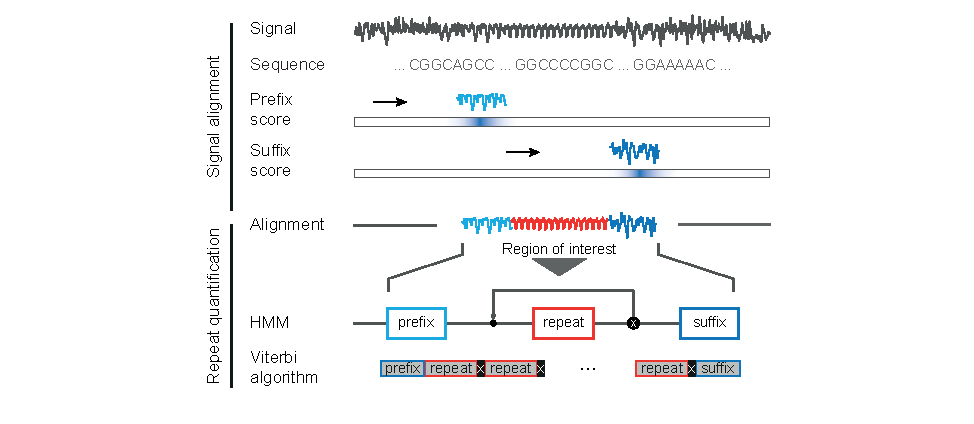
\includegraphics[width=1.0\textwidth]{figures/strique/count_structure_plasmid.pdf}
	\captionsetup{format=plain}
	\caption[\textit{STRique}: generic repeat detection pipeline on raw nanopore signals.]{Repeat quantification enabled by raw signal alignment of flanking prefix and suffix regions and HMM-based count on the signal of interest.}
	\label{fig:strique:count_structure_plasmid}
\end{figure}

\begin{figure}[h]
	\centering
	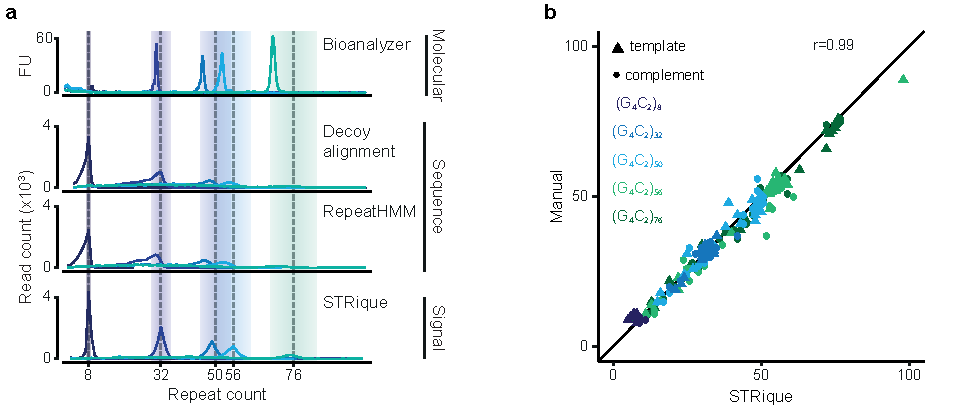
\includegraphics[width=1.0\textwidth]{figures/strique/count_signal_corr.pdf}
	\captionsetup{format=plain}
	\caption[Correlation and strand bias in STR analysis methods]{\textbf{a}, Bioanalyzer electropherogram, decoy alignment, \textit{RepeatHMM} and \textit{STRique} counts of synthetic $ (G_{4}C_{2})_{n} $ repeats. \textbf{b}, Manual counted set of plasmid reads on y-axis correlating with \textit{STRique} raw signal pipeline on x-axis. Only data points shown which could also be evaluated with methods in Fig. \ref{fig:strique:count_seq_manual} (n=15, 49, 45, 48, 47; Pearson correlation).}
	\label{fig:strique:count_signal_corr}
\end{figure}

\begin{figure}[h]
    \centering
    \includegraphics[width=1.0\textwidth]{figures/strique/count_bac.pdf}
    \captionsetup{format=plain}
    \caption[Strand bias in sequence based repeat counts]{Comparison of repeat counts from \textit{STRique}, decoy alignment based on guppy (high accuracy model, 16k window size) and repeatHMM based on guppy (high accuracy model, 16k window size) for BAC data. One dot (n=5004) per read passing all three approaches and colored by strand.}
    \label{fig:strique:count_bac}
\end{figure}


\subsection{Repeat expansion in C9orf72 and FMR1}
\label{subsec:strique:c9orf72}

\begin{itemize}
	\item application to patient data
	\item Cas9 enrichment to increase on-target coverage
	\item C9orf72 and FMR1 repeat counts
\end{itemize}

Previously, repeat instability had been noted in Bacterial Artificial Chromosomes (BAC) containing expanded C9orf72 $ [(G_{4}C_{2})_{n}] $-repeats (Online Methods).17 Analysing BAC clone 239 from a c9FTD/ALS patient (G4C2)~800 (Ref. 17) with \textit{STRique}, we observed STR contractions in many reads and a secondary peak at 800 repeats (Fig 1d, Online Methods), while all evaluated sequence space based methods failed to mirror previously published Southern blot results (Fig.1d, Supplementary Fig. 5). 17


Next, to establish a baseline reference data set, we performed nanopore sequencing of a whole genome library from c9FTD/ALS patient-derived DNA yielding a total of 29 Gbp from a single MinION flow cell. Consistent with approximately 10-fold genome-wide coverage, 10 reads covered the C9orf72 target region. To improve the coverage of any predetermined STR, but particularly the (G4C2)n-region in our proof of concept study, we took advantage of the programmable CRISPR-Cas12a-ribonucleoprotein (Cas12a-RNP), which cleaves DNA via staggered double-strand breaks.23 The Cas12a-RNP was first applied to selectively target DNA sequences from a patient-derived induced pluripotent stem cell line (24/5\#2) adjacent to the (G4C2)n-repeat resulting in unique 4 bp overhangs as molecular tags amenable to ligation of a linker oligo and subsequent attachment of the nanopore sequencing adapter (Fig. 2a: Workflow I, Online Methods). To further improve enrichment results we replaced the oligo adapter ligation step by adding Klenow fragment to fill in the Cas12a overhangs. The resulting dA-tailed DNA ends enabled even more efficient ligation of the sequencing adapters. In this enrichment protocol variant, the phosphorylated 5’-ends generated by Cas-nuclease mediated cleavage provide the molecular tag for selectively ligating the nanopore sequencing adaptors to the targeted DNA fragment (Fig. 2a, Workflow II).
Additional dephosphorylation of all 5’-ends before Cas12a-RNP-digestion chemically protects DNA ‘background’ fragments from being ligated to sequencing adapters. Consequently, only those fragments cut by Cas12a-RNPs are capable of being sequenced by this procedure (Fig. 2a). As a result, we were able to obtain up to 82 reads covering the (G4C2)n-repeat including 40 reads from the expanded allele from a single MinION flow cell (Supplementary Fig. 7, Supplementary Table 3, Supplementary Note). Strikingly, consistent with Southern blot results from the same cell line (Supplementary Fig. 8 a,b), we found two distinct repeat expansion distributions (Fig. 2b). To further explore the general applicability of our enrichment, sequencing and signal processing protocol to other repeat expansion disorders, we tested two isogenic, patient-derived cell lines (SC105iPS6, SC105iPS7) carrying distinct FMR1-repeat expansions.24 Employing an new set of FMR1-targeting Cas12a-RNPs (Supplementary Table 1) we found two different repeat expansion distributions as predicted by Southern blot analysis (Fig. 2c, Supplementary Fig. 8 c,d).
Since other CRISPR/Cas-nucleases also generate phosphorylated 5’-ends after DNA cleavage,25 we explored, if nucleases such as Cas9 might enable additional improvements of the enrichment results. Therefore, we prepared libraries in parallel with Cas12a- and Cas9-RNPs targeting both FMR1 and C9orf72 regions. Remarkably Cas9-targeting results in an additional increase in sequencing depth in the order of a magnitude for both targeted regions concomitant with a notable reduction in off-target reads (Fig. 2d, Supplementary Fig. 7c). To understand, if the number of reads on target can be further improved by exposing the same Cas12a- or Cas9- enrichment library to an increased number of pores, we subjected equimolar aliquots from the same pooled library preparations from Fig. 2b to nanopore sequencing on PromethION flow cells, which contain on average six times as many nanopores. However, we did not observe a gain in reads on target with the larger flow cells (Supplementary Fig. 7c).

\begin{figure}[h]
    \centering
    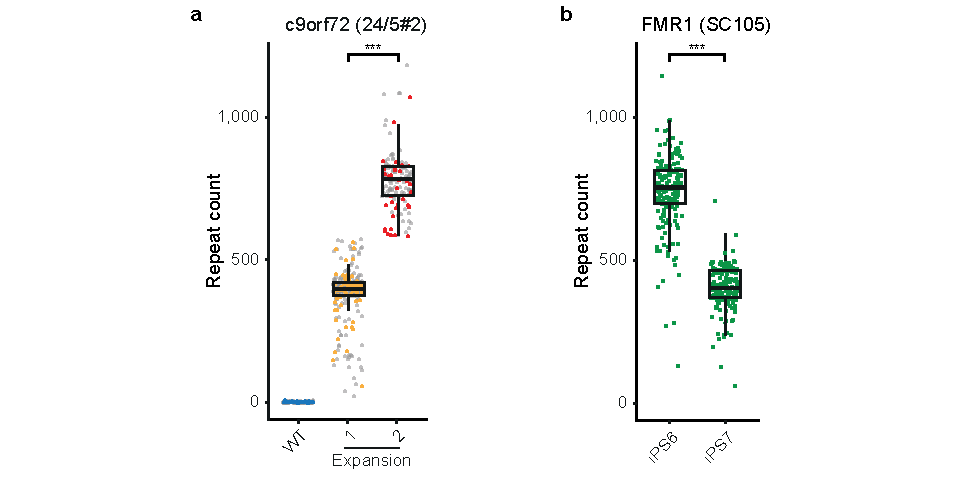
\includegraphics[width=1.0\textwidth]{figures/strique/count_patient_samples.pdf}
    \captionsetup{format=plain}
    \caption[Repeat quantification in c9orf72 and FMR1 patients]{\textbf{a}, Repeat quantification of sample 24/5\#2 at the C9orf72 locus, revealing two distinct repeat bands of ~450 and ~750 $ (G_{4}C_{2})_{n} $ repeats (n = 1,810, 738 and 363 evaluated reads with a difference in repeat length of 392 (95\% confidence interval (CI): 383 to 400), $ P < 2.2 \cdot 10^{-16} $). Colored points indicate reads used in Fig. \ref{fig:strique:methylation_c9orf72_region}b. WT, wild type. \textbf{b}, Repeat quantification of the SC105iPS6 and SC105iPS7 samples at the FMR1 locus (n = 174 and 168 evaluated reads with a difference in repeat length of -343 (95\% CI: -361 to -325), $ P < 2.2 \cdot 10^{-16} $). P values in a and b were obtained by a two-sided Wilcoxon rank-sum test; $ ***P < 0.001 $. Data are presented as boxplots (centerline, median; box limits, first and third quartiles; whiskers, 1.5x interquartile range).}
    \label{fig:strique:count_patients}
\end{figure}

\begin{figure}[h]
    \centering
    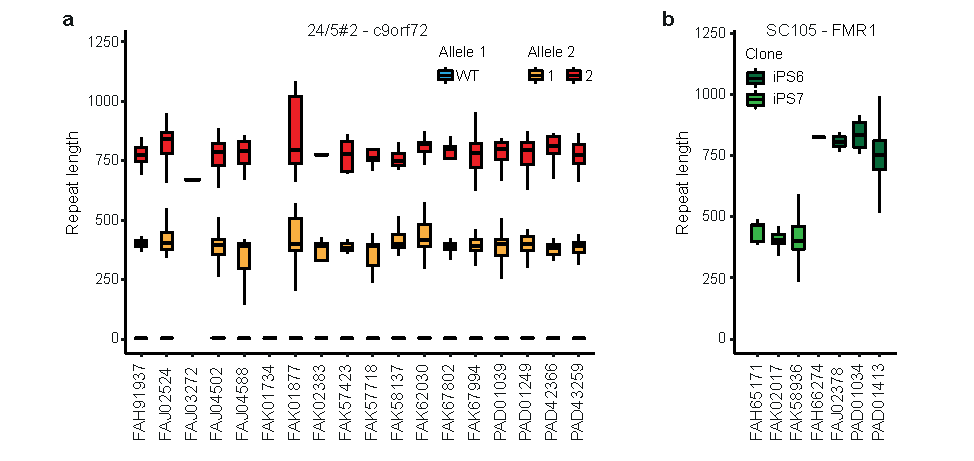
\includegraphics[width=1.0\textwidth]{figures/strique/count_experiments.pdf}
    \captionsetup{format=plain}
    \caption[Repeat count cluster stability over experiments]{\textbf{a}, C9orf72 target enrichment flow cells for patient 24/5\#2 \textbf{b}, FMR1 enrichment flow cells of SC105iPS6/iPS7. (FA*: MinION, PAD*: PromethION, number of reads per boxplot are in Supplementary Tables 5-6 column wt and exp). Data presented as boxplots (centerline, median; box limits, first and third quartiles; whiskers, 1.5x interquartile range; outliers not shown)}
    \label{fig:strique:count_experiments}
\end{figure}




\section{Methylation detection}
\label{sec:strique:modifications}


\subsection{Region methylation detection}

\begin{itemize}
	\item region methylation detection in masked reads with nanopolish
	\item verification in BAC boundaries
\end{itemize}

\subsection{Repeat methylation detection}

\begin{itemize}
	\item extension of signal algorithm by twin-HMM for multiple pore models
	\item repeat methylation detection by STRique
	\item verification in MSssI methylated plasmid
\end{itemize}

The epigenetic modification of C9orf72 and FMR1 loci have been correlated with STR expansion status and patient characteristics in both disorders, however without quantification at the single molecule level so far.10,26 Therefore we integrated single read CpG methylation analysis of regions adjacent to both STRs using nanopolish14 with our \textit{STRique} results (Fig. 3a). We found that in the 24/5\#2 line all reads with STR expansions > 750 repeats showed a significantly increased methylation level at the promoter CpG island. In contrast all wild type reads and those with ~450 repeats were not or only partially methylated (Two sided Wilcoxon rank sum test p < 0.001, Fig. 3b, Supplementary Fig. 9, Supplementary Note).
Additionally, in c9FTD/ALS patients pervasive CpG methylation of the (G4C2)n-repeat itself has been reported.27 Assessed with a strictly qualitative assay, the expanded STR itself was reported to be methylated in the majority of cases examined.27 A similar observation has been directly implicated in the pathogenesis of FXS, where a CGG repeat expansion at the FMR1-locus beyond a threshold of > 200 repeats leads in most cases to the silencing of the entire FMR1-gene through CpG-methylation.28
Due to the intrinsic heterogeneity in STR length, especially reference genome based methods such as nanopolish14 cannot be used to determine CpG methylation on the repeat expansion itself. To detect 5mC modifications on STRs, we extended \textit{STRique} by employing a parallel HMM with unmodified- and 5mC-paths. This single read analysis returns a methylation state for each tandem repeat, which then can be summarized into the mean repeat methylation level over the whole repetitive sequence.
When applying the methylation-aware \textit{STRique}, all expanded FMR1-STRs in nanopore reads from patient SC105 are found to be highly methylated (Supplementary Fig. 10a), consistent with previous analyses29 and our Southern blot results (Supplementary Fig. 8). We next evaluated this approach on plasmids containing n=76 synthetic (G4C2)n and n=99 CGG-repeats (Addgene, \#63089), which were covalently modified with the methyltransferase M.SssI (Supplementary Fig. 10).14 In addition we tested the algorithm on (G4C2)n-containing reads (online methods) from patient-derived DNA, which had been modified with M.SssI in vitro. In summary, we found that \textit{STRique} can determine the repeat CpG methylation state correctly in all positive and negative controls evaluated.
Surprisingly though, all reads covering the C9orf72-STR from our patient-derived samples showed little to no CpG-methylation, independently of the repeat expansion length or methylation status of the promoter CGI (Fig. 3b).


\begin{figure}[h]
    \centering
    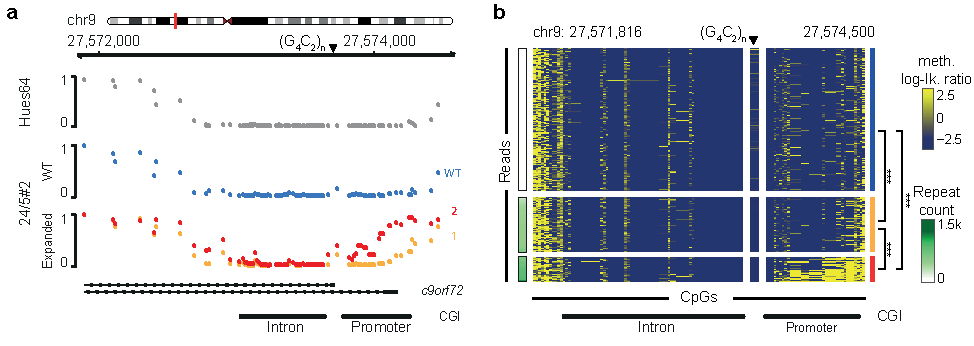
\includegraphics[width=1.0\textwidth]{figures/strique/methylation_c9orf72_region.pdf}
    \captionsetup{format=plain}
    \caption[Methylation state analyses at the single-read level]{\textbf{a}, C9orf72 methylation status in HUES64 as measured by whole-genome bisulfite sequencing. The wild-type (blue) allele and expanded (ex; orange) alleles (with 450 and 750 $ (G_{4}C_{2})_{n} $ repeats (red), respectively) are shown for patient 24/5\#2, as measured by nanopore sequencing. \textbf{b}, Single read nanopore methylation of C9orf72 covering reads from the minus strand (n = 259, 100 and 43 rows per block) sorted by detected repeat length (rows, single read; columns, single CpGs). CpGs with logP ratio $> 2.5$ are considered methylated, while those with logP ratio $< -2.5$ are considered unmethylated. The median methylation difference (95\% CI) and P value (determined by two-sided Wilcoxon rank-sum test on mean promoter CGI methylation) for comparisons were as follows: $ WT-ex450: 3.9 \cdot 10^{-5} (4.8 \cdot 10^{-6} to 3.4 \cdot 10^{-2}), P = 5.3 \cdot 10^{-9}; WT-ex750: 0.56 (0.46-0.64), P < 2.2 \cdot 10^{-16}; ex450-ex750: 0.53 (0.40-0.64), P < 2.2 \cdot 10^{-16}; ***P < 0.001. $ }
    \label{fig:strique:methylation_c9orf72_region}
\end{figure}

\begin{figure}[h]
    \centering
    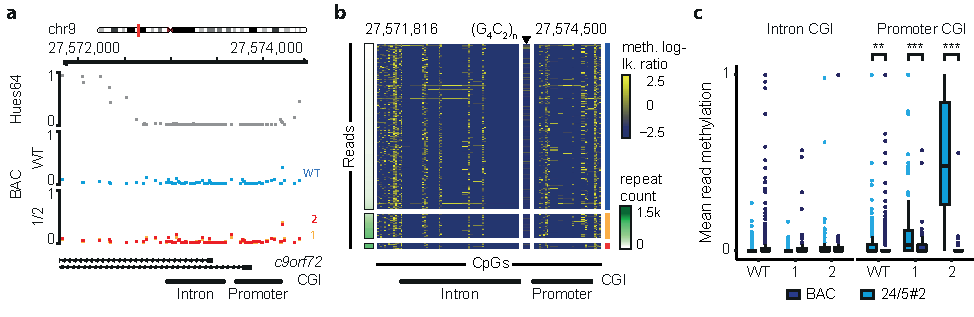
\includegraphics[width=1.0\textwidth]{figures/strique/methylation_bac_region.pdf}
    \captionsetup{format=plain}
    \caption[Nanopore single read methylation in BAC data]{\textbf{a}, Methylation status of c9orf72 region in BAC data for repeats < 200 (WT), 200-750 (Cluster1,orange) and > 750 (Cluster2,red) and control (Hues64, WGBS) \textbf{b}, Single read methylation on a sample of 500 BAC minus strand reads sorted by repeat count (row split 200 and 750 repeats, n=423,63,14). \textbf{c}, Difference in mean CGI methylation of intron and promoter per read on minus strand. Reads binned by detected repeat length for BAC (n=2066 WT; 315 Cluster1; 72 Cluster2) and patient 24/5\#2 (n=925 WT; 362 Cluster1; 153 Cluster2). Two sided Wilcoxon rank sum test, corrected for multiple testing (Holm), q-vals: * 0.05 - 0.01; ** 0.01 - 0.001; *** < 0.001. Median methylation differences between promoter CGI [95\%CI] for WT $-2.3e^{-5} [CI: -5.6e^{-6}:-1.5e^{-5}, q=7.4e^{-3}] $ and Cluster1 $ -0.01 [CI: -7.1e^{-5}:-3.4e^{-2}, q=1.4e^{-17}] $ and Cluster2 $ -0.46 [CI: -0.58:-0.37, q=1.0e^{-26}] $.}
    \label{fig:strique:methylation_bac_region}
\end{figure}

\begin{figure}[h]
    \centering
    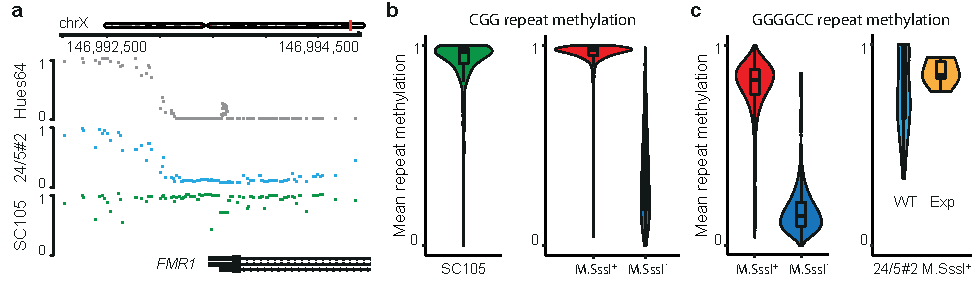
\includegraphics[width=1.0\textwidth]{figures/strique/methylation_repeat.pdf}
    \captionsetup{format=plain}
    \caption[Region and repeat methylation detection]{\textbf{a}, FMR1 region methylation in SC105iPS6/iPS7 compared to Hues64 WGBS and patient sample 24/5\#2. \textbf{b}, CGG mean repeat methylation status detected by \textit{STRique} for SC105 (n=197) and synthetic plasmid control with 99 repeats treated with $ M.SssI^{+/-} $ (5mC level on minus strand, n=1232 $ M.SssI^{+} $; n=11991 $ M.SssI^{-} $). \textbf{c}, GGGGCC repeat methylation status for plasmid control with 76 repeats treated with $ M.SssI^{+/-} $ (n=2939 $ M.SssI^{+} $; n=31280 $ M.SssI^{-} $) and patient sample 24/5\#2 treated with $ M.SssI^{+} $ (5mC level on minus strand, n=52 WT and n=6 Cluster1). Data in (b-c) presented as violin plots with overlayed boxplots (centerline, median; box limits, first and third quartiles; whiskers, 1.5x interquartile range; outliers not shown).}
    \label{fig:strique:methylation_repeat}
\end{figure}




\section{Summary}
\label{sec:strique:summary}

Our results demonstrate the precise and multi-layered molecular characterization of pathological short tandem repeat expansions. We have increased the enrichment for regions of interest on the background of the human genome approximately two orders of magnitude without any target amplification by using selective, multiplexed CRISPR/Cas-nuclease-based chemical tagging of DNA fragments. Importantly, our method does not require any additional instruments in contrast to other previously reported30 enrichment strategies and enables reporting the DNA methylation status of the same alleles. The CRISPR/Cas-nuclease-target enrichment and \textit{STRique} can be rapidly adapted to any other genomic region of interest, ensuring broad applicability to overcome challenges associated with the single molecule analysis. This allows for immediate integration of genetic and epigenetic signals associated with unstable repeat expansions or any other as of yet unsequenceable genomic regions in human health and disease. This type of analysis improves diagnostic workflows in regard to accuracy and resolution of unstable repeat expansion while enabling efforts to gain mechanistic insights into effects on differentiation, aging and future therapeutic agents that modify DNA methylation.



	\chapter{Discussion}
\label{cha:summary}

\textit{But could you not also do that with short reads?} - Expressing an initial scepticism against a novel technology, nanopore sequencing is, six years after the first release in 2014, still termed the emerging technology.
Next-generation sequencing remains the established and widely undisputed reference method.
However, after significant improvements, addressing shortcomings of throughput and accuracy, both third-generation platforms have evolved to become the primary technology for genome assembly and are commonly used for the analysis of viral and bacterial genomes.
Yet, a broader replacement of NGS methods is not in sight, raising the question, why the introductory question is not more frequently re-phrased to: \textit{Would nanopore here not be the more suitable platform?} Or: \textit{Would you not confirm this by using nanopore sequencing?}

The underlying research question of this work is therefore to analyze unique use-cases for nanopore sequencing, identify key limitations and provide a comprehensive investigation of the current status.
Despite many improvements, the application of nanopore sequencing in the context of large mammalian and plant genomes remains challenging.
At the same time are the benefits of long reads known: Reliable alignments in repetitive regions, no duplicates and biases by library amplification and the linkage of distant genetic and epigenetic features on single molecule level.
Yet, the stable throughput, higher read accuracy and established workflows of NGS technologies justify the commitment to nanopore sequencing only for applications infeasible with short reads.

A niche to gain traction at applying nanopore sequencing is the analysis of repetitive regions in the human genome.
For comparison, using short reads, the reachable part of a repeat is limited by the read length, leading to ambiguous alignments, once a read contains only repeat sequence.
Short tandem repeats (STRs) are accumulations of three to six nucleotide long sequence patterns, in disease cases expanded to hundreds of copies.
The epigenetic analysis of repeats is a unique feature of nanopore sequencing, considering that SMRT sequencing is not sufficiently sensitive to 5-methylcytosine on single-molecule level.
Repeat detection by sequencing is the digital advancement over southern blot based quantification, increasing the accuracy and reducing the turnaround time.
\textit{STRique} is a bioinformatic analysis software, developed to integrate the quantification of short tandem repeats with their methylation state on individual read level.
The algorithmic key features of \textit{STRique} are raw signal alignment and the sequence to signal annotation.
Due to the oversampling of the sequencer, raw signal traces are roughly ten times longer compared to their corresponding sequence and, with respect to noise and time warping, generally more difficult to handle.
Yet, only a signal based counting algorithm allows to bypass systematic errors induced during conventional basecalling of tandem repeats.
Hidden Markov Models (HMM) are a powerful resource to align nanopore signals to a reference sequence, with the most prominent usage in the \textit{Nanopolish} package.
However, their computational complexity is scaling quadratically with the number of hidden states, limiting the usage to restricted signal and sequence windows of interest.
The purpose of the signal alignment is therefore, to extract a signal segment covering the repeat with sufficient flanking sequence to anchor a counting HMM.
The flexibility of the HMM is needed over a static alignment, since the repeat length is unknown and varying between reads.
A looping transition around a single repeat profile allows the model to iterate through an arbitrary number of repeat patterns.
The signal alignment is the enabling and at the same time limiting step: The Viterbi path through the HMM is the most likely state-sequence given the observed signal, fed with a wrong signal alignment, the model will still yield a repeat count.
A filtering based on signal alignment scores is therefore crucial to exclude low quality counts.
A useful side-effect of the signal alignment is the ability to mask regions within the read.
\textit{STRique} provides a script to cut out the expanded repeat from the raw signal and creates wild-type like reads passing any conventional downstream pipeline, to detect for instance DNA-methylation in the repeat-flanking sequence.
Taken together, \textit{STRique} is an example for a unique nanopore application, enabling more detailed investigations of short tandem repeat expansions.

Bioinformatics for nanopore sequencing are undergoing constant development.
In contrast to NGS analysis, even a stable nanopore workflow needs constant maintenance to factor in accuracy improvements, but also recent file format and compression method changes.
Zooming out from individual tool to pipeline level, the streamlined processing and data archiving has received very little attention in the nanopore community.
Computational setups ranging from few MinION flow cells analyzed on a Laptop to high-throughput PromethION sequencing in combination with GPU accelerated cluster environments are complicating, if not inhibiting, a uniform vendor provided processing strategy.
The motivation behind the development of the \textit{Nanopype} pipeline is therefore not only to wrap the processing, but also set up a scaling data management.
While certainly site specific on the implementation detail, the concepts of the pipeline backend transfer to any institute aiming to set up a nanopore workflow.
The ONT sequencing software \textit{MinKnow} is providing raw data in batches of currently 4k reads packed into \textit{fast5} files.
Further transfer to permanent storage, indexing and archiving are essential for a high-throughput environment.
The organization in batches is, as opposed to a single \textit{fastq} file per NGS run, beneficial for distributed processing.
\textit{Nanopype} operates on batches whenever possible, submitting for instance alignments in batches bears the advantage that multiple compute nodes can process a single sequencing run and that only few reads need to be re-processed in case of errors.



Nanopype: Processing to stay up to date with updating software
storage to handle raw data, x times larger than fastq from NGS
snakemake over shell scripts for modularity, supporting container, multiple cluster backends
Build and functionality tests are very rare!
Interchangeable tools for lab focused on development
weakness: trying to maintain increasing number of integrated tools and their dependencies, example pytorch/tensorflow v1/v2 for neural networks
Future work: freeze core pipeline, develop NanopypeXT which uses Nanopype as sub-workflow for very specific or complex to maintain tools

Literature: Throughput and accuracy increasingly suitable for application to large plant and mammalian genomes
Assembly and structural variant detection are established but will further benefit from accuracy and even longer reads
Limitations on wet-lab side with high molecular weight DNA and amount of input material
Limitations on bioinformatic, storage and upload, refer to STRique data being in Figshare repository
Base modification visibility long known, lack of robust and accurate tools
RNA modifications example of frequently mentioned potentials with only few applications up to date

Future work based on pipeline backend and baseline set with signal annotation
Base modification framework on event data without dependency to basecaller generation
Base caller based on novel transformer neural networks with impressive results in translation and speech to text








	\cleardoublepage
	
	% --------------------------
	% Appendix
	% --------------------------
	\appendix
	\chapter{Nanopype Supplement}
\label{cha:supplement:nanopype}

\section{Listings}
\label{sec:supplement:nanopype:listings}
\lstinputlisting[language=bash, caption=Snakemake installation wrapper, label=lst:nanopype:build]{listings/nanopype/snakemake_build.txt}

%\label{sec:supplement:nanopype:listings}
%\lstinputlisting[language=yaml, caption=Nanopype environment configuration example, label=lst:nanopype:env]{listings/nanopype/env.txt}

%\label{sec:supplement:nanopype:listings}
%\lstinputlisting[language=yaml, caption=Nanopype workflow configuration example, label=lst:nanopype:workflow]{listings/nanopype/nanopype.txt}




\section{Report}
\label{sec:supplement:nanopype:report}
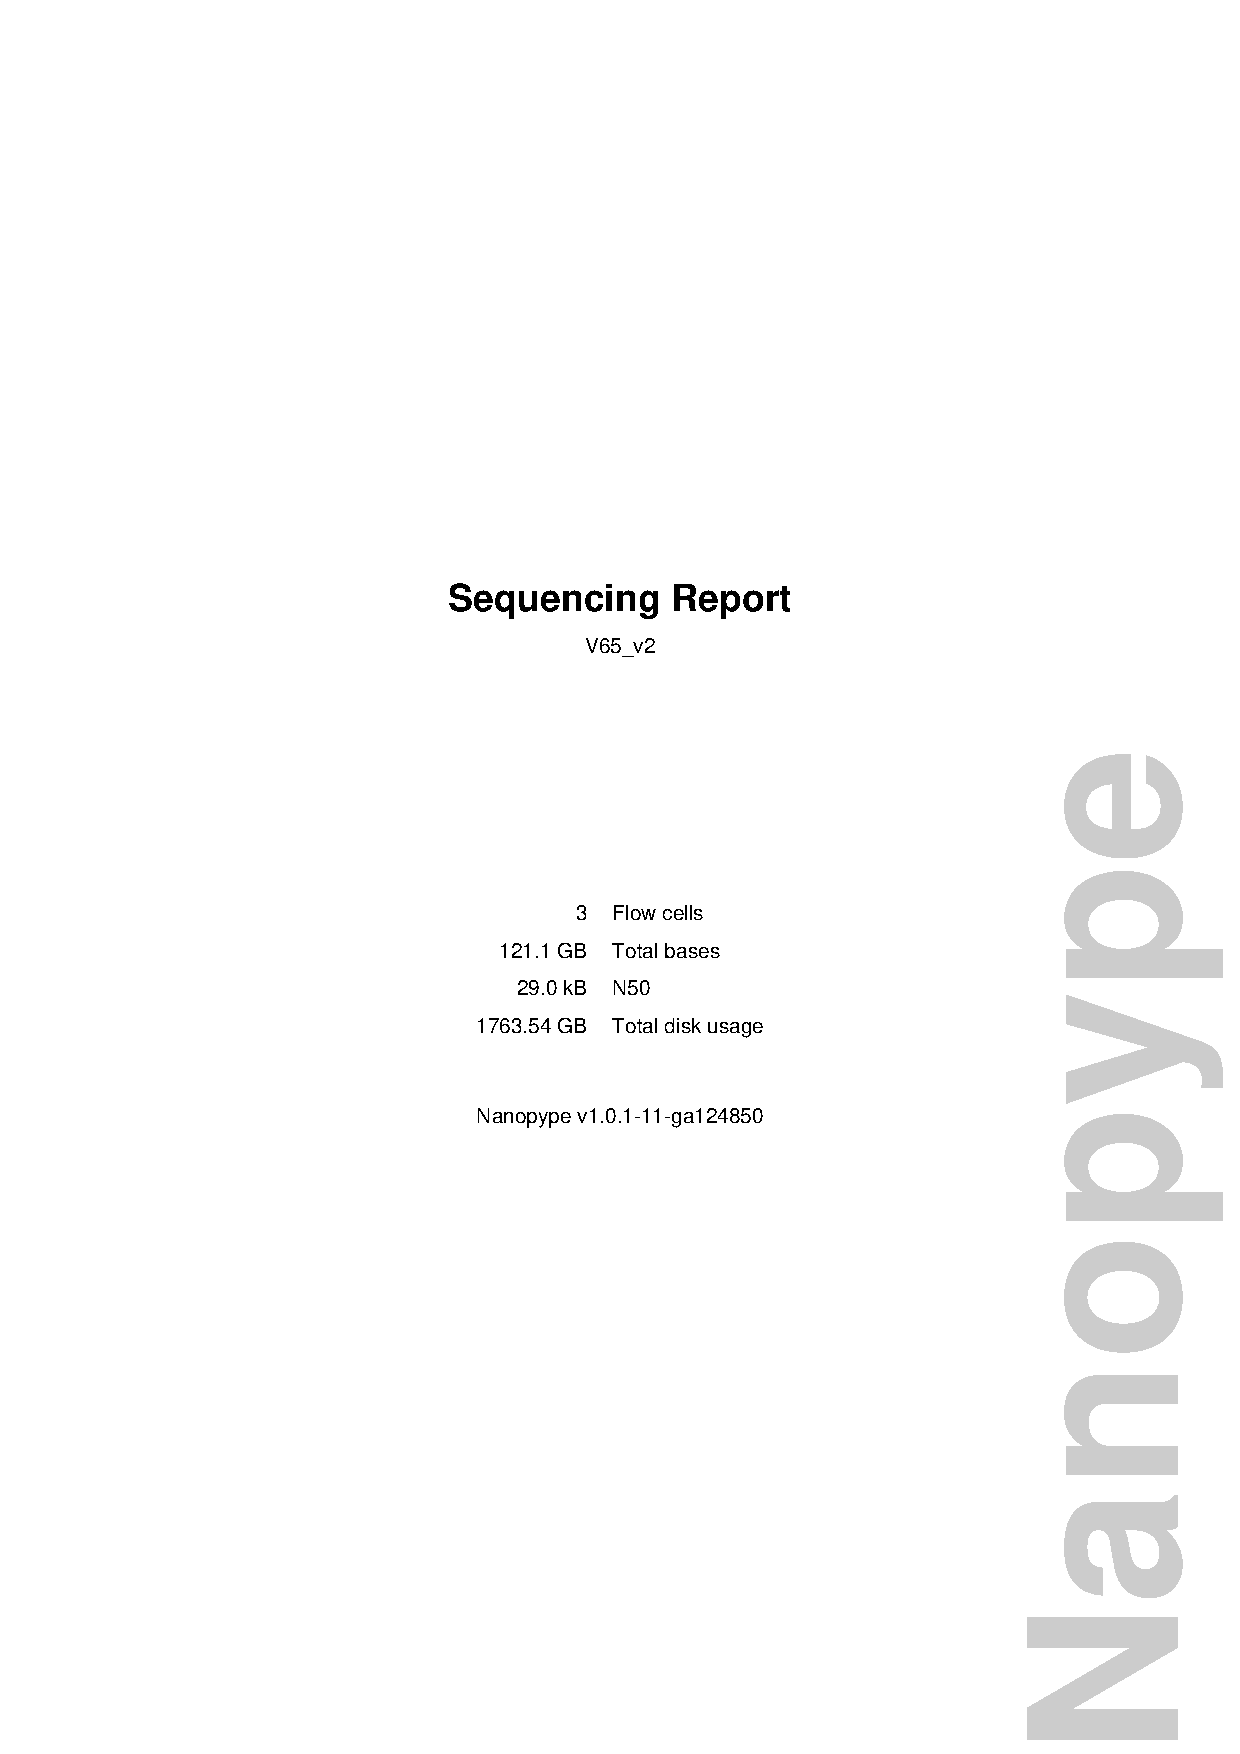
\includepdf[pages=-]{figures/nanopype/V65.pdf}

	\cleardoublepage
	
	% --------------------------
	% Back matter
	% --------------------------
	{%
		\setstretch{1.1}
		\renewcommand{\bibfont}{\normalfont\small}
		\setlength{\biblabelsep}{10pt}
		\setlength{\bibitemsep}{0.5\baselineskip plus 0.5\baselineskip}
		\printbibliography
		%\printbibliography[nottype=online]
		%\printbibliography[heading=subbibliography,title={Websites},type=online,prefixnumbers={@}]
	}
	\cleardoublepage
	
	\listoffigures
	\cleardoublepage
	
	\listoftables
	\cleardoublepage
    
    \renewcommand{\lstlistlistingname}{List of Listings}
    
    \lstlistoflistings
    \cleardoublepage 
	
	%\clearpage
	%\newpage
	%\mbox{}
	
	%************************************************
% Declaration
%************************************************
\pdfbookmark[0]{Declaration}{Declaration}
\chapter*{Declaration of Authorship}
\label{sec:declaration}
\thispagestyle{empty}

I declare to the Freie Universität Berlin that I have completed the submitted dissertation
independently and without the use of sources and aids other than those indicated. The present
thesis is free of plagiarism. I have marked as such all statements that are taken literally or in
content from other writings. This dissertation has not been submitted in the same or similar form in
any previous doctoral procedure.
I agree to have my thesis examined by a plagiarism examination software. 

\bigskip

\noindent\textit{\thesisUniversityCity, \thesisDate}

\smallskip

\begin{flushright}
	\begin{minipage}{5cm}
		\rule{\textwidth}{1pt}
		\centering\thesisName
	\end{minipage}
\end{flushright}

%*****************************************
%*****************************************

	\cleardoublepage
	
	\pagestyle{empty}
\hfill
\vfill
\pdfbookmark[0]{Colophon}{Colophon}
\section*{Colophon}

This thesis was typeset with \LaTeXe.
It uses the \textit{Clean Thesis} style developed by Ricardo Langner.
The design of the \textit{Clean Thesis} style is inspired by user guide documents from Apple Inc.

%Download the \textit{Clean Thesis} style at \url{http://cleanthesis.der-ric.de/}.

	\cleardoublepage
	% **************************************************
	% End of Document CONTENT
	% **************************************************
\end{document}
